\chapter{Aufgabe 1}
\section{Textsatzbeschreibungssprachen}
Mit dem Begriff \textit{Satz} wird ein technisches Verfahren beschrieben mit dem aus einer Vorlage, eine drucktaugliche Form hergestellt wird.
Diese können händische, maschinelle oder computergestütze Verfahren sein.
Ziel des Textsatz ist es ein Dokument \textbf{ästhetisch ansprechend} und \textbf{leicht leserlich} zu formatiern.
Dafür werden zum Beispiel Schriftarten und das Seitenlayout festgelegt\cite{satzwiki:2023}.
Diese Prinzip wird auch mit \textit{What you see is what you ask for (WYSIWYAF)} umschrieben.\par
Es gibt verschiedene Textsatzbeschreibungssprachen.
TeX wurde 1978 von Donald E. Knuth entwickelt und LaTeX\cite{latex:2023} ist ein von Leslie Lamport für TeX\cite{tex:2023} entwickeltes Softwarepaket, das die Benutzung von \textbf{TeX vereinfacht}.
Für Unix wurde 1990 das Textsatzsystem Groff von James Clark veröffentlicht.
Dort wird es genutzt um \textit{manpages}(Bedienungsanleitungen) darzustellen\cite{groff:2022}.
Markdown ist ebenfalls eine Textsatzbeschreibungssprache die 2004 von John Gruber und Aaron Schwartz veröffentlicht wurde.
Der Grundgedanke bei Markdown ist es \textbf{einfach lesbar und schreibbar} zu sein\cite{lasar:2013}.
1988 wurde die Seitenbeschreibungssprache Ghostscript von Peter Deutsch veröffentlicht.
Ghostscript ist ein Interpreter der als \textit{Programmierschnittstelle} dient, um PostScript und PDF-Inhalte darzustellen und diese drucken zu können\cite{ghostscript:2022}. 

\section{Vergleich Textsatzbeschreibungssprachen und Programmiersprachen}
Ähnlichkeiten zwischen Textsatzbeschreibungssprachen und Programmiersprachen findet man sehr häufig. 
Die verwendeten Pakete oder bei Programmiersprachen Bibliotheken werden zu beginn der Datei eingebunden.
In LateX könnte man den Befehl:
\begin{lstlisting}
\begin{document} 

\end{document}
\end{lstlisting}

mit der Hauptfunktion in C-Programmen vergleichen:

\begin{lstlisting}
int main(){

} 
\end{lstlisting}
Befehle wie in einer Programmiersprache lassen zudem bestimmte Formatierungen auf den Text ausführen.
Unterschiedlich ist allerdings, dass in Textsatzbeschreibungssprachen der Text auch \textbf{einfach runter geschrieben} werden kann, wo hingegen in Programmiersprachen ein Befehl angegeben werden muss um Text auszugeben.

\section{Unterschiede zu integrierten Wortprozessoren}
Integrierte Wortprozessoren arbeiten nach dem Prinzip \textit{What you see is what you get (WYSIWYG)}\cite{wysiwyg:2023}.
Dies bedeutet dass die Darstellung auf dem Bildschirm in \textbf{Echtzeit} stattfindet.
Ein Beispiel dafür ist in Abbildung \ref{Wortprozessor} zu sehen.
Genutzt wird dies zum Beispiel bei \textit{HTML-Editoren} um Personen mit \textbf{wenig HTML-Kenntnissen} das editieren von Webseiten zu ermöglichen.

\begin{figure}[h]
	\centering
	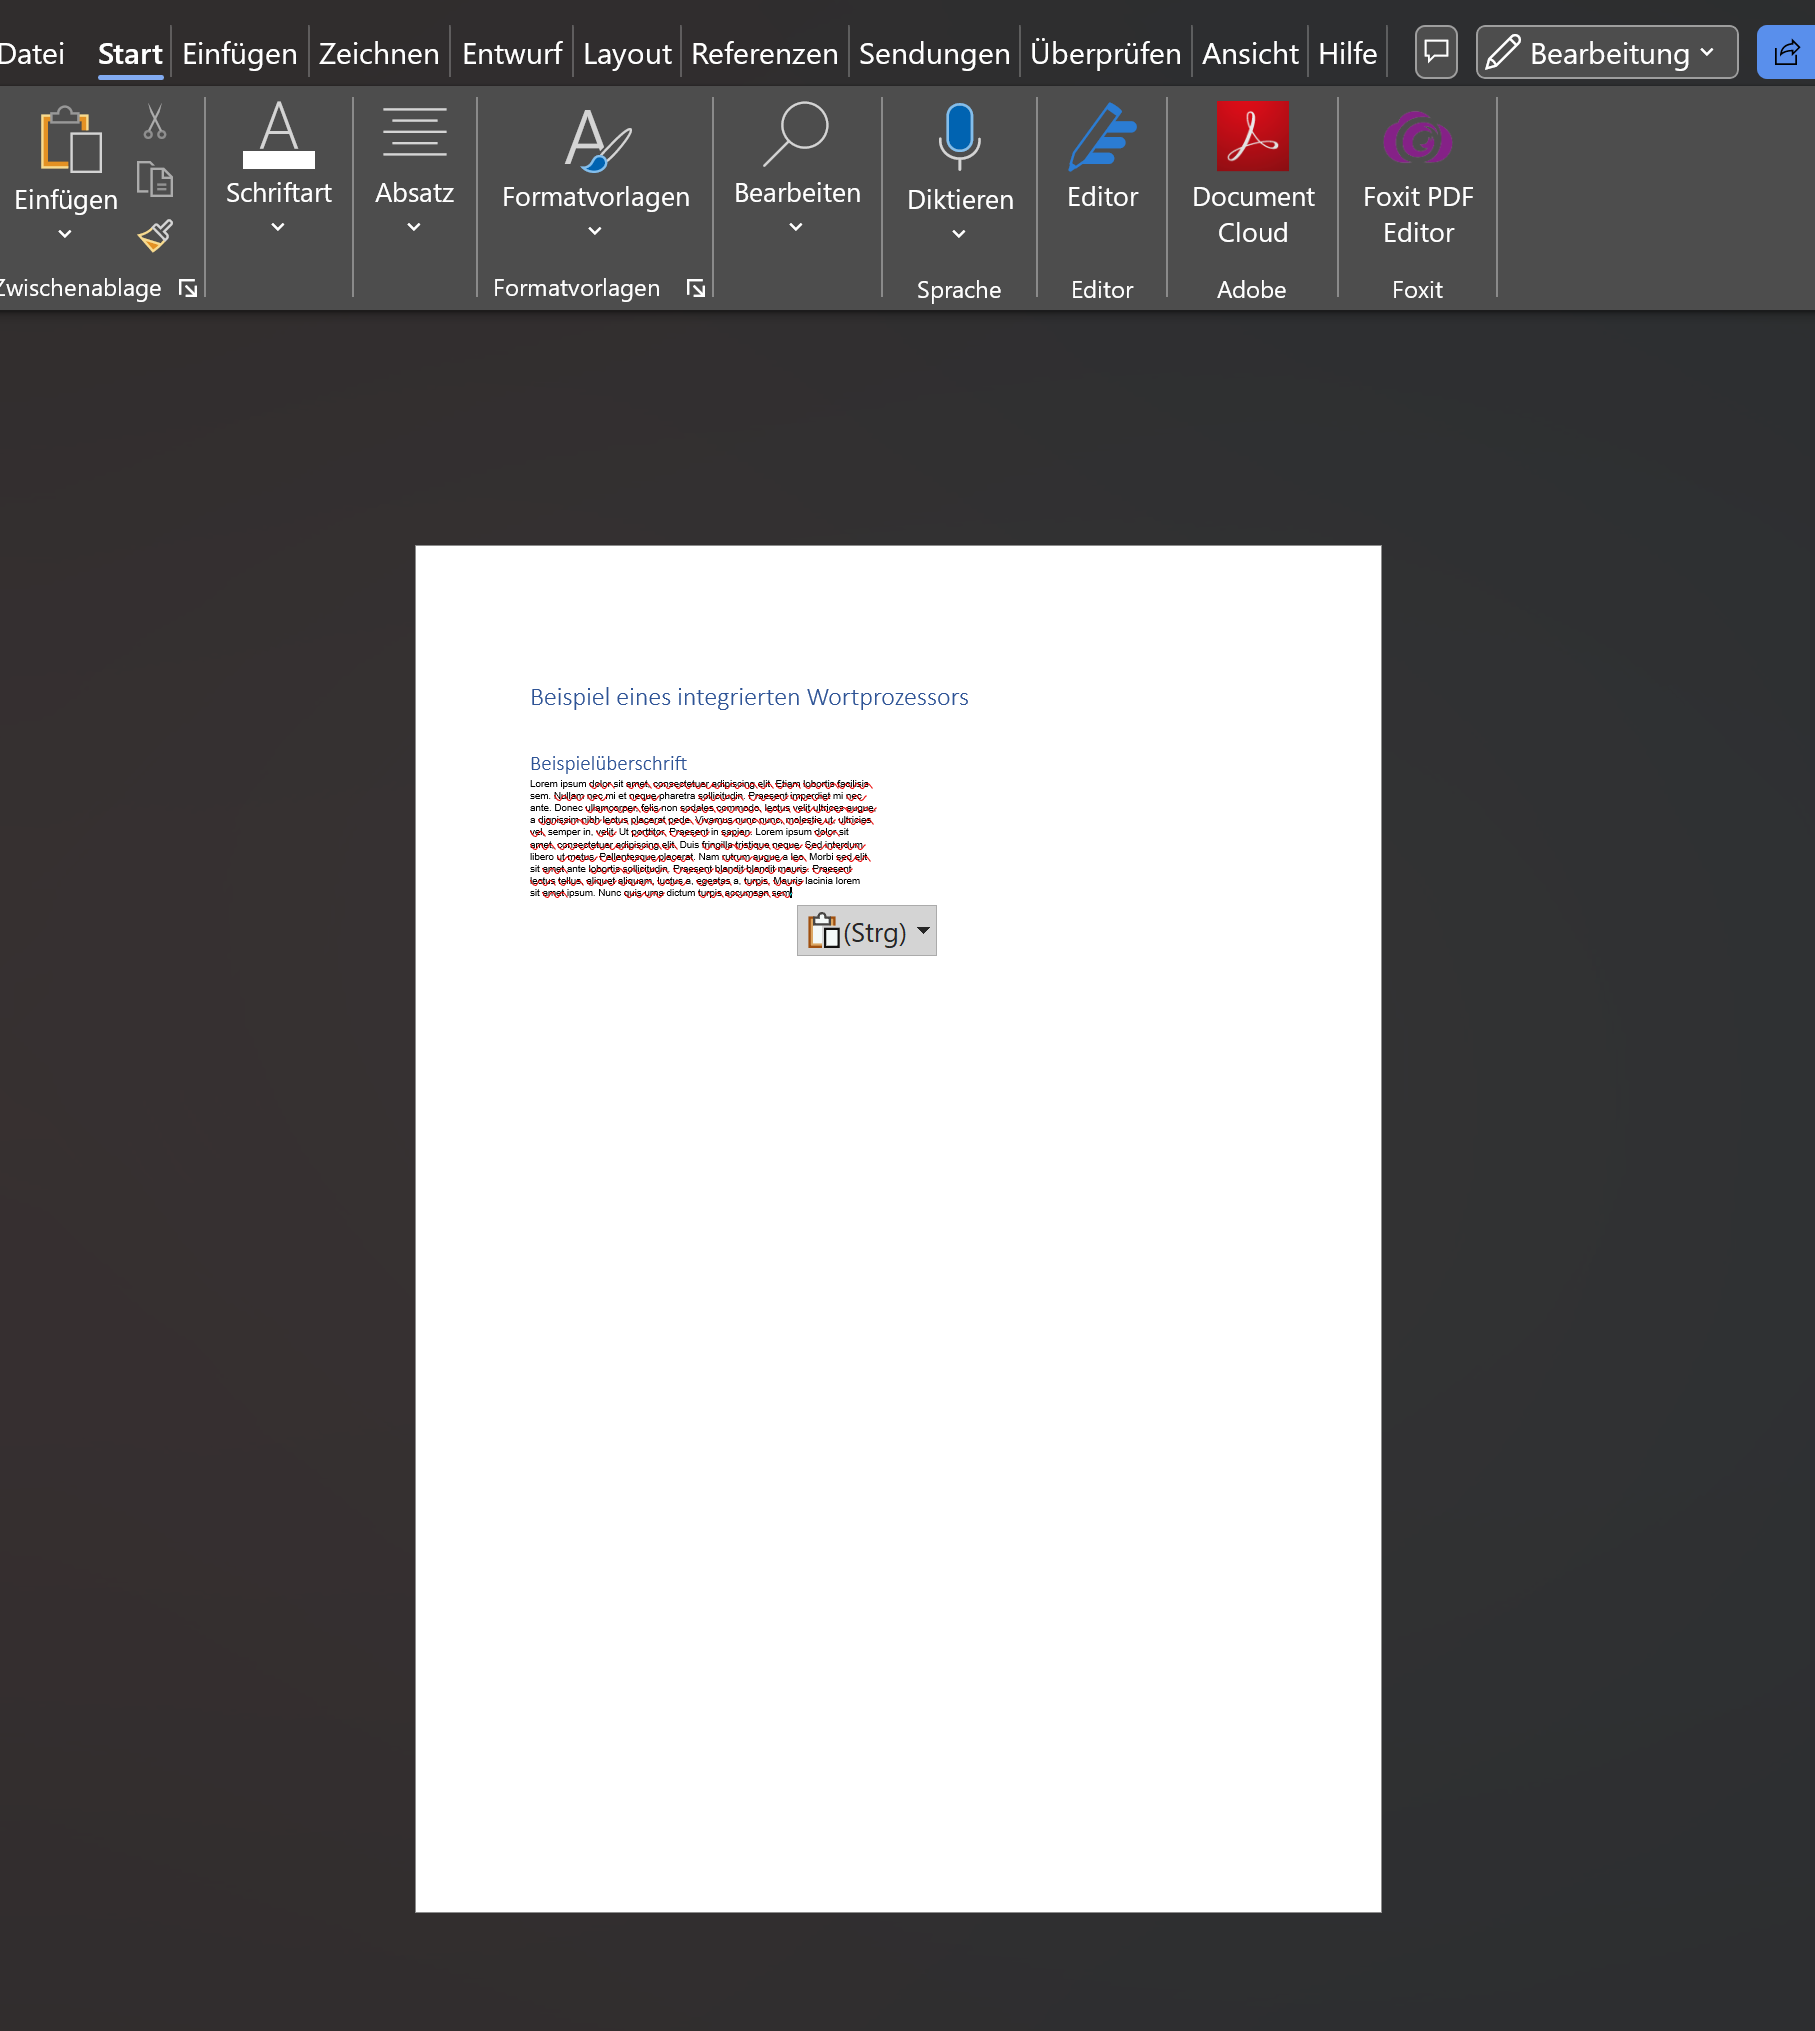
\includegraphics[scale=0.5]{Images/Wortprozessor.png}
	\caption{Beispiel eines integrierten Wortprozessors in dem Programm Word}
	\label{Wortprozessor}
\end{figure}

Textsatzbeschreibungssprachen setzen hingegen auf das bereits erwähnte WYSIWYAF-Prinzip.
Dabei werden innerhalb des Textes Formatierungseinstellungen ausgezeichnet und sich folglich die Ein- und Ausgabe unterscheidet, wie in Abbildung \ref{VergleichLaTeX} zu sehen ist.
Dies erfordert allerdings eine \textbf{längere Einarbeitungszeit} als das WYSIWYG-Prinzip.
Dies bringt aber auch Vorteile mit sich.
Textsatzbeschreibungssprachen sind häufig rechnerunabhängig.
Auch eignen sich Textsatzbeschreibungssprachen für das erstellen von größeren Dokumentationen.
LaTeX ist darauf ausgelegt gut gestaltete Dokumente mit einheitlicher Formatierung zu gestalten, die auch nachträglich auf Dokumente anwendbar sind\cite{schweitze:2013}.\par 

\begin{figure}[h]
	\centering
	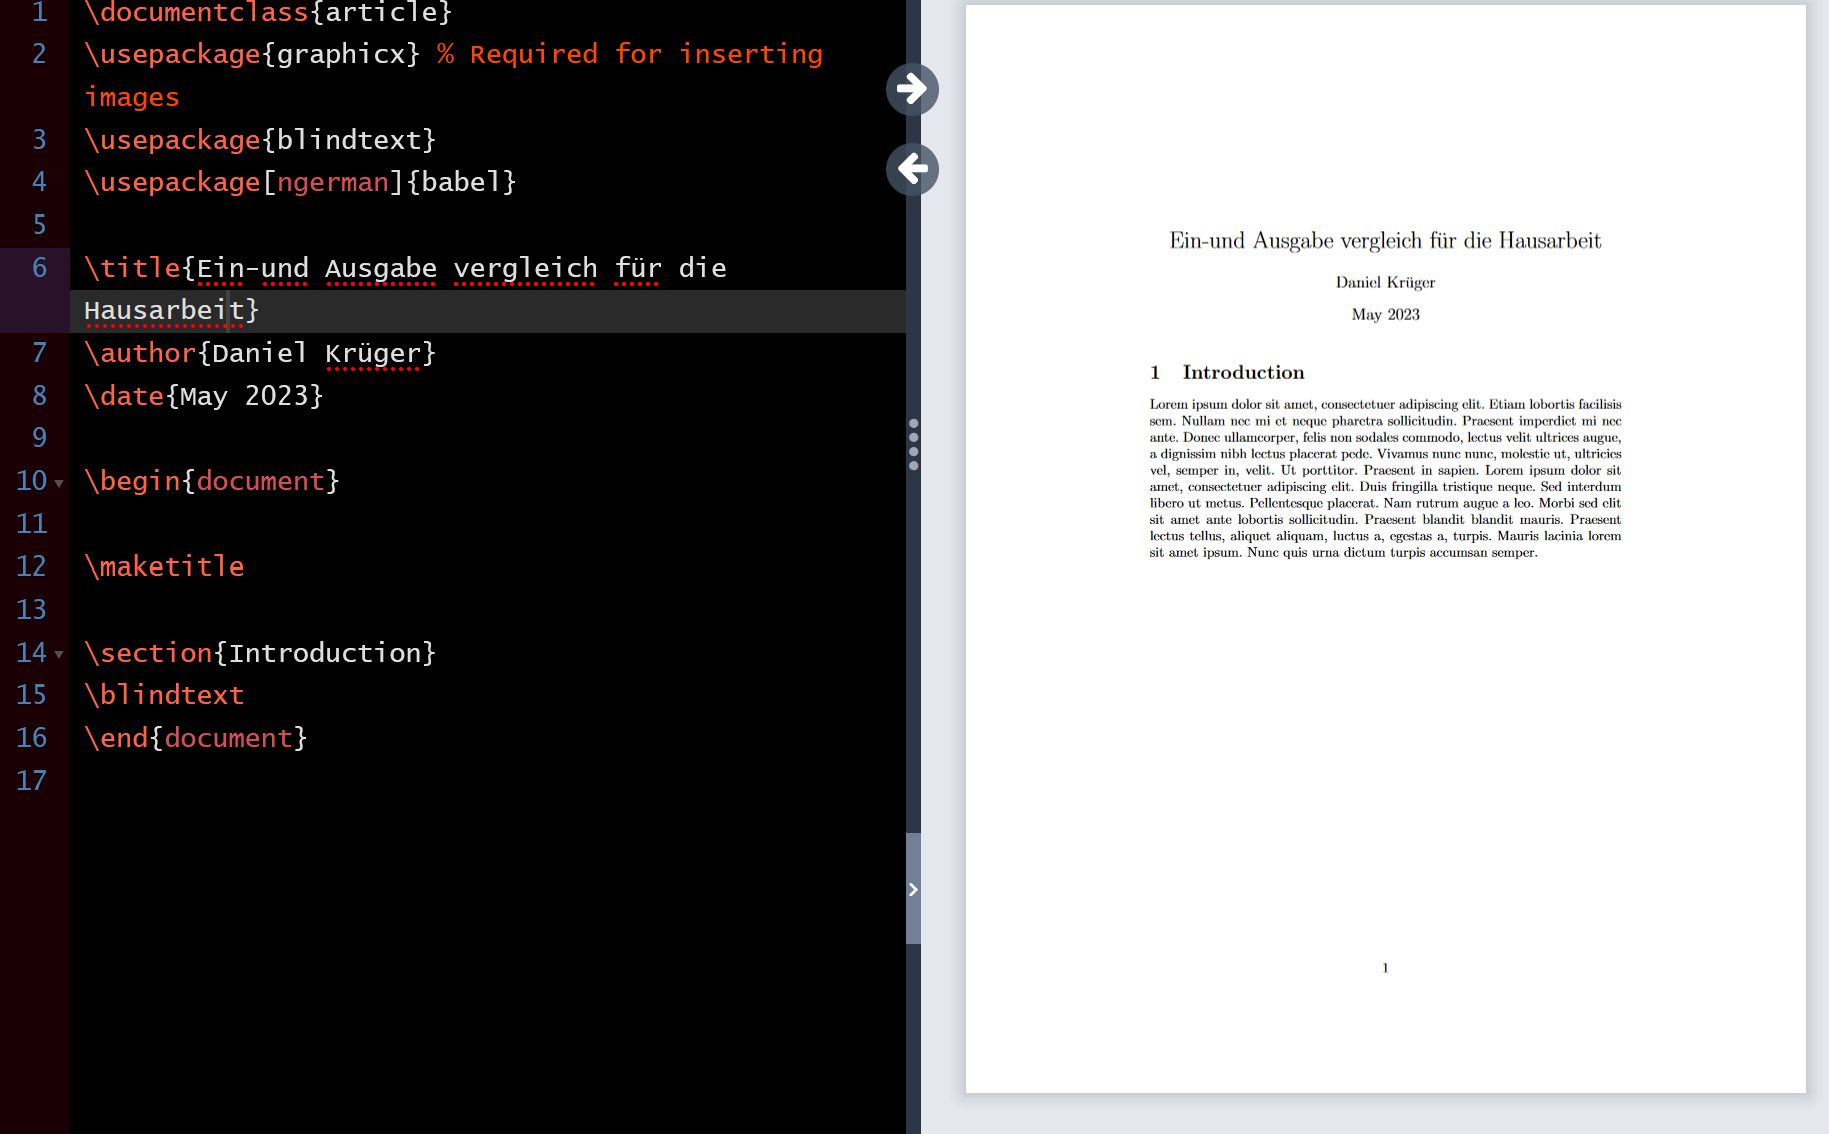
\includegraphics[scale=0.5]{Images/Vergleich_LaTeX.png}
	\caption{Beispiel einer Textsatzbeschreibungssprache mit Ein- und Ausgabe von LaTeX}
	\label{VergleichLaTeX}
\end{figure}

